\documentclass{resume} % Use the custom resume.cls style

\usepackage[left=0.75in,top=0.6in,right=0.75in,bottom=0.6in]{geometry} % Document margins
\usepackage{xcolor}
\usepackage{hyperref}
\hypersetup{
    colorlinks=true,
    linkcolor=blue,
    filecolor=magenta,      
    urlcolor=teal,
}
\usepackage{graphicx}
\newcommand{\tab}[1]{\hspace{.2667\textwidth}\rlap{#1}}
\newcommand{\itab}[1]{\hspace{0em}\rlap{#1}}
\name{Emilio Berti} % Your name
\address{
    \centering
    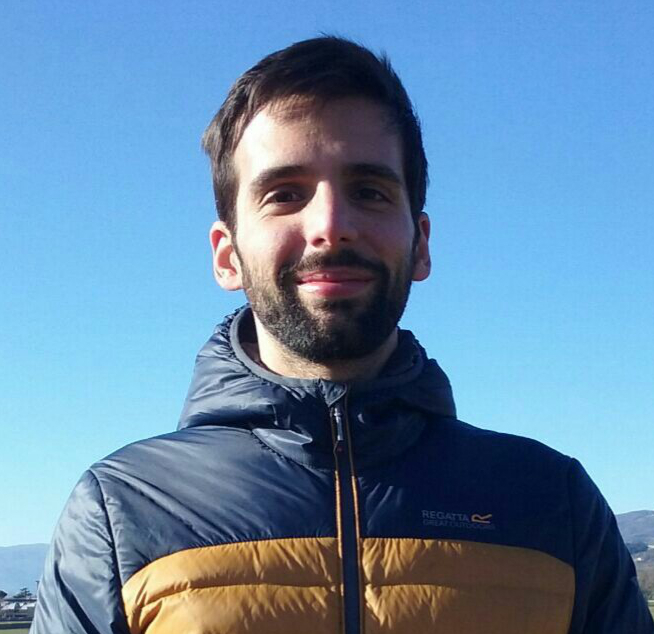
\includegraphics[width=0.25\textwidth]{Emilio.jpg}
} % Your address
%\address{123 Pleasant Lane \\ City, State 12345} % Your secondary addess (optional)
\address{(+45) 266 54 662 \\ emilio.berti90@gmail.com} % Your phone number and email

\begin{document}

\begin{rSection}{Summary}
I am a theoretical ecologist with a passion for math and computing.
I am a very fast learner and I have worked in many different fields of biology, from the microscopic scale of muscle physiology to the global scale of vertebrates macroecology.
I have an strong quantitative background, with expertise in mathematical and statistical modelling of complex systems using big databases at large spatio-temporal scales.
I have a comprehensive knowledge of traditional statistical methodologies, e.g. linear regression, and with cutting-edge algorithms such as machine learning.
I have outstanding programming skills, particularly in optimizing large computations using Geographic Information Systems (GIS).
I am fluent in writing and spoken English skills and I have good communication skills in scientific and daily settings.
I can propose and develop new ideas independently and have a very collaborative personality.
\end{rSection}

\begin{rSection}{Work History}

{\bf PostDoctoral researcher} \hfill {\em October 2020 -- Present}\\
Theory in Biodiversity Sciences\\
German Centre for Integrative Biodiversity Research (\textsc{iDiv})\\
Leipzig, Germany

{\bf Scientific consultant} \hfill {\em May 2020 -- July 2020}\\
Department of Bioscience\\
Aarhus University\\
Aarhus, Denmark

{\bf Teaching assistant} \hfill {\em February 2017 -- April 2020}
\\Department of Biology\\
Aarhus University\\
Aarhus, Denmark
\end{rSection}

\begin{rSection}{Education}
{\bf PhD} \hfill {\em February 2017 -- June 2020} 
\\ Section of Ecoinformatics and Biodiversity
\\ Department of Biology
\\ Aarhus University
\\ Aarhus, Denmark\\
\\ {\bf Visiting PhD student} \hfill {\em Fall 2018}
\\ Department of Ecology and Evolution
\\ University of Chicago
\\ Chicago, IL\\
\\ {\bf MSc cum laude in Biology} \hfill {\em 2013 -- 2016}
\\ Department of Ecology and Evolution
\\ University of Florence
\\ Florence, Italy\\
\\{\bf BSc in Biology} \hfill {\em 2009 -- 2012}
\\ Department of Physiology
\\ University of Florence
\\ Florence, Italy
\vskip3ex
\end{rSection}

\begin{rSection}{Postgraduate courses}
{\bf ``Species Distributions Modelling''} \hfill {\em 2019}\\
Evora, Portugal -- Lecturers: Prof. Miguel Ara\'{u}jo and Dr. Babak Naimi\\
{\bf ``Megafauna ecology -- shaping past, present and future ecosystems.''} \hfill {\em 2019}\\
Aarhus, Denmark\\
{\bf ``Mixed models''} \hfill {\em 2019}\\
Aarhus, Denmark -- Lecturer: Prof. Rodrigo Labouriau\\
{\bf ``Writing and Speaking Science in English for Biology Students''} \hfill {\em 2019} \\
Aarhus, Denmark -- Lecturer: Prof. Brian Sorrell \\
{\bf ``Ecosystem roles of megafauna in the past, present, and future''} \hfill {\em 2017}\\
Aarhus, Denmark\\
{\bf ``Mediterranean School of Complex Networks (MSCx)''} \hfill {\em 2017} \\
Salina, Italy
\end{rSection}

\begin{rSection}{Skills}
{\bf Language}\\
Italian (native), English (fluent), Danish (beginner)\\
{\bf Programming}\\
R (expert), bash (expert), python (proficient), C (proficient), julia (proficient), sqlite (proficient), html (proficient)\\
{\bf Software} \\
Linux/GNU, Rstudio, Juno, Anaconda, Jupyter, QGIS, \LaTeX, Markdown, Pandoc, Git version control, GitHub, Bitbucket, Overleaf\\
{\bf Methods} \\
Statistics, regression analysis, effect sizes, mixed models, variables selection, PCA, ordination and classification, optimization, machine learning, network analysis, mathematical modelling, extrapolation and forecasting, species distribution models, environmental niche modeling, spatial modeling, geographic information systems (GIS), demographic projections, quantitative genetic, big data, data visualization, data science, APIs, automation. 
\end{rSection}

\begin{rSection}{Teaching \& Organized Workshops}
{\bf Teaching Assistant} \\
Statistical and Geospatial Modelling (2019)\\
Behavioural Biology (2018, 2019)\\
Geographic Information System (2017)\\
{\bf Organized Workshops}\\
``Cleaning online repository data for use in biogeography and macroecology'' (2019)\\
``Running a species distribution model in R.'' (2019)\\
``A (very) gentle introduction to Linux.'' (2019)
\end{rSection}

% \begin{rSection}{References}
% \textbf{Jens-Christian Svenning} (Professor)\\
% Aarhus University, Department of Biology, Ecoinformatics and Biodiversity\\
% E-mail: svenning@bios.au.dk
% Phone: +45 289 92 304

% \textbf{Robert Buitenwerf} (Assistant Professor)\\
% Aarhus University, Department of Biology, Ecoinformatics and Biodiversity\\
% E-mail: buitenwerf@bios.au.dk\\
% Phone: +45 871 54 346

% \textbf{Giacomo Santini} (Assistant Professor)\\
% Florence University, Department of Biology\\
% E-mail: giacomo.santini@unifi.it\\
% Phone: +39 055 45 74 721
% \end{rSection}

\begin{rSection}{Publications}
% \vspace{4ex}\hfill{\em 2020}\\
\textbf{Berti, E.} \& Svenning, J.C. (2020). Megafauna extinctions have reduced biotic connectivity worldwide. \textit{Global Ecology and Biogeography}. DOI: \href{https://doi.org/10.1111/geb.13182}{10.1111/geb.13182}.

\textbf{Berti, E.}, Monsarrat, S., Munk, M., Jarvie, S., \& Svenning, J.C. (2020). Body size is a good proxy for vertebrate charisma. \textit{Biological Conservation}. DOI: \href{https://doi.org/10.1016/j.biocon.2020.108790}{10.1016/j.biocon.2020.108790}.
\end{rSection}

\begin{rSection}{Links}
\begin{minipage}{0.5\textwidth}
\begin{itemize}
    \item \href{https://scholar.google.com/citations?user=5KPh-oUAAAAJ&hl=en}{Google Scholar profile}
    \item \href{https://emilio-berti.github.io/}{Personal website}
    \item \href{https://orcid.org/0000-0001-9286-011X}{ORCiD}
\end{itemize}
\end{minipage}
\begin{minipage}{0.5\textwidth}
\begin{itemize}
    \item \href{https://www.linkedin.com/in/emilio-berti-55a348146}{LinkedIn}
    \item \href{https://github.com/emilio-berti}{GitHub}
\end{itemize}
\end{minipage}
\end{rSection}

\end{document}
